\chapter{Vorgehen Performanceanalyse}
\section{Motivation}

Die Performance respektive Leistungsfähigkeit einer Applikation stellt einer der bedeutendsten Qualitätsanforderungen dar. Sie kann nich nur zu verärgerten Benutzern, sondern auch zu einer Verlangsamung der Business-Prozesse führen. Die Motivation für eine Performanceanalyse entsteht, wenn die in Service Level Agreement oder Anforderungsanalyse spezifizierten \textbf{Qualitätsanforderungen nicht erfüllt} sind. Optimal wäre, wenn diese Anforderung während des Entwicklungsprozesses kontinuierlich geprüft würde.

\section{Ablauf}
Die Performanceanalyse ist ein iterativer Prozess und sollte so lange dauern, bis die Anforderungen erfüllt und der Kunde zufrieden ist. Sie besteht aus folgenden vier Schritten\cite{hummelBeer201109}:
\begin{enumerate}
	\item Identifikation der neuralgischen Punkte des Systems
	\item \textbf{Suche nach dem Dominating Consumer\footnote{Kirk Pepperdine bezeichnet die Aktivität, welche dominiert wie die CPU gebraucht wird, als Dominating Consumer . }}
	\item \textbf{Sammeln von Detaildaten}
	\item Lösen des Problems
\end{enumerate}


Damit die Analyse der Garbage Collection zum richtigen Zeitpunkt gemacht wird, sind insbesondere die Punkte zwei und drei wichtig. Sie werden in den folgenden beiden Abschnitten genauer definiert.
\section{Suche nach dem Dominating Consumer}\label{dominating_consumer}
Die Suche nach dem Dominating Consumer kann nach folgendem Schema durchgeführt werden:
\begin{figure}[H]
  	\centering
    	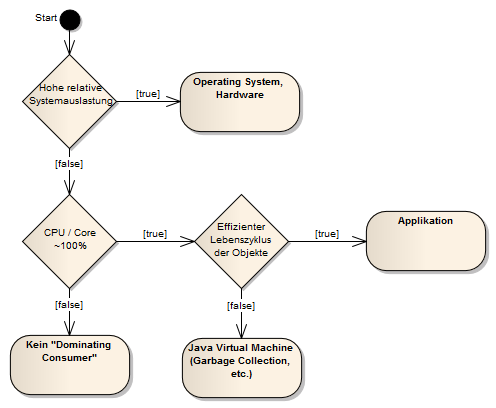
\includegraphics[width=13.1cm]{images/dominating_consumer}
        	\caption{Suche nach dem Dominating Consumer}
\end{figure}

\subsection{Hohe relative Systemlast}\label{hohe_systemauslastung}
Die erste Frage, die sich bei der Suche nach dem Dominating Consumer stellt, ist, ob die hohe CPU-Auslastung\footnote{CPU kann auch einer oder ein paar Cores bedeuten.} durch die Applikation oder das System verursacht wird. Je nach Betriebssystemen gibt es dafür unterschiedliche Werkzeuge:
\begin{itemize}
	\item \textbf{Windows:} Task Manager / Lasche Performance (Leistung). Für die Anzeige der Systemzeit muss die Anzeige der Kernelzeit eingeblendet werden: View / Show Kernel Times
	\item \textbf{Linux / Unix: } vmstat zeigt die Ausnutzung der CPU: vmstat 5
\end{itemize}

Hohe Systemauslastung kann unterschiedliche Gründe haben: 
\begin{itemize}
\item \textbf{Exzessives Context-Switching\footnote{Kontextwechsel}:} Mehrere Prozesse können sich die gleiche CPU (CPU-Kern) nur deshalb teilen, weil beim Wechsel von Prozess A auf B ein Context-Switch gemacht wird, so dass Thread B am selben Ort weiterarbeitet wo er beim letzten Mal war. Gründe für exzessives Context-Switching können beispielsweise nicht adäquat gewählte Locks sein. Wenn ein Thread aufgrund der Synchronisation angehalten werden muss.\footnote{Symptomatisch zeigt dann vmstat, das System ist nicht im Leerlauf, aber die Kernelzeiten (cpu/sy) dominieren die Zeit des Benutzers (cpu/us).}
\item \textbf{Hohe I/O Festplatte} 
\item \textbf{Hohe I/O Netzwerk} 
\end{itemize}


\subsection{Hohe CPU- respektive Core-Last}
Sofern die im Abschnitt \ref{hohe_systemauslastung} beschriebenen Punkte nicht zutreffen, stellt sich die Frage, ob die Auslastung der CPU überhaupt gross ist. Ist das nicht der Fall, gibt es womöglich gar keinen Dominating Consumer - es muss dann herausgefunden werden, was die Threads weg von der CPU haltet. Es gibt dafür laut \cite{pepperdine201102} unterschiedliche Gründe:
\begin{itemize}
\item \textbf{Dead Locks: } Threads schliessen sich gegenseitig aus. 
\item \textbf{Applikation skaliert nicht: } Applikation hat schlechte multi-core Eigenschaften.
\item \textbf{Langsame Disks / Netzwerke}
\item \textbf{Zu kleine Connection- und Thread-Pools}
\item \textbf{Aurufe auf langsame externe Systeme}
\end{itemize}


\subsection{Effizienter Objekt-Lebenszyklus}
Sofern die relative Systemlast klein und die CPU-Auslastung gross ist, muss der Lebenszyklus der Objekte angeschaut werden. Dies kann auf unterschiedliche Arten getan werden:
\begin{itemize}
\item \textbf{Memory Analyse: }Es wird angeschaut, wie alt die Objekte in den verschiedenen Bereiche (Young Collection, Old Collection) sind. Wieviele Garbage Collection Zyklen sie überlebt haben.
\item \textbf{Garbage Collection: }Wann und wie oft werden Garbage Collections durchgeführt, wie lange haben sie gedauert, wieviel Speicher haben sie befreit.
\end{itemize}

\section{Sammeln von Detaildaten}
Je nach Dominating Consumer müssen weitere Daten gesammelt oder andere Analysen gemacht werden. Die folgenden beiden Abschnitte gehen tiefer in die Grundlagen der Garbage Collection ein und zeigen die Eigenheiten der JRockit Virtual Machine.


